
\section{結果と考察}
\subsection{各用途に合わせた原子配列の表示結果}
\subsubsection{削除された原子の識別表示}
原子の削除操作は,岩佐の研究で最安定の原子配列の構造を探索するために取り入れた手法である.
boundary modelerで2223などと指定して作成された原子配置では,真ん中と両端にある粒界近傍で原子位置の極端に近いペアが生成する.このままでは,高いエネルギーとなり緩和がうまく進行しない.そこで,boundary adjusterで原子の削除を行う.削除前後のPOSCARを比較して原子位置を特定する作業をVESTAなどでは手動で行うが,この削除された原子の位置を視覚的に把握しやすくするための表示法を工夫した.なお,以下のコードを入力することでsafari上に表示される.
\begin{lstlisting}[style=customCsh,basicstyle={\scriptsize\ttfamily}]
% ruby viewer.rb POSCAR_2223 POSCAR_2223_4
% open -a safari view.svg 
\end{lstlisting}
原子の削除有無を識別した三面図は,図\ref{fig:010}のように表示される.

\begin{figure}[htbp]\begin{center}
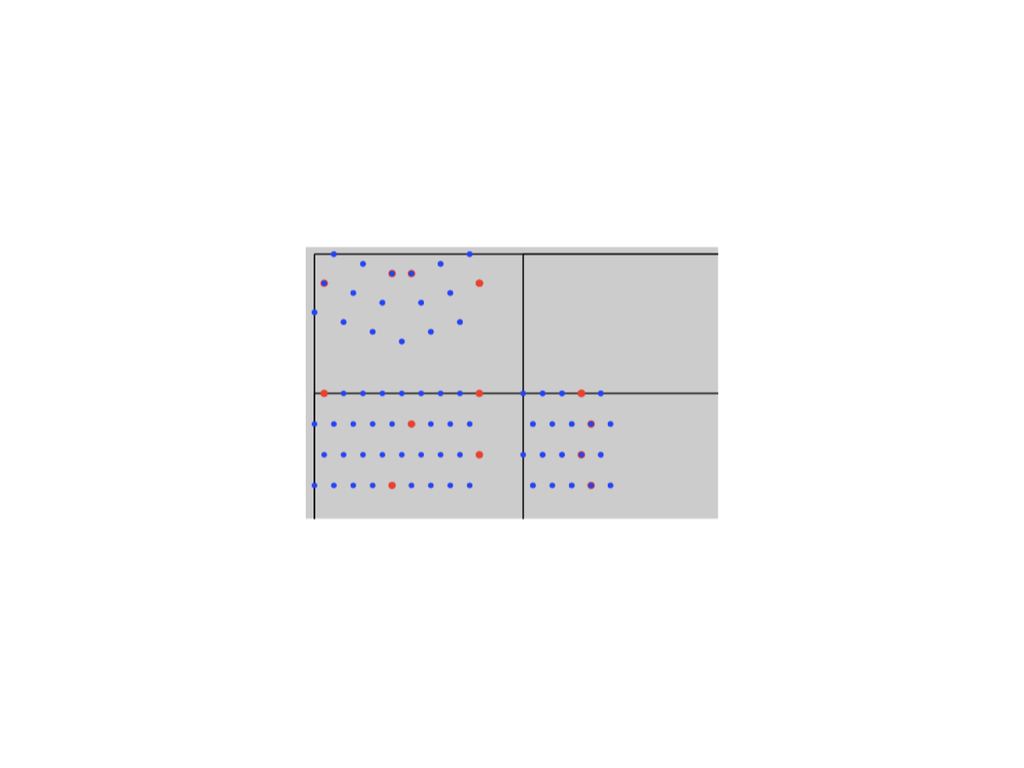
\includegraphics[width=10cm,bb= 0 0 937 753]{../figs/./boundary_narita.010.jpeg}
\caption{削除前後のPOSCARを色分けした三面図.}
\label{fig:010}
\label{default}\end{center}\end{figure}

図中の赤い丸が削除された原子に相当する.
平面図では青と赤が重なっているが,これは正面図からわかる通り,上下に重なった原子位置で削除の有無が存在するためである.
VESTAなどの汎用ソフトでは,このような操作は標準で用意されておらず,原子種を変えるなどの工夫によって表示することが必要である.
しかし,開発したviewerでは二つのPOSCARの原子位置から自動で判定するようにしている.
また,三面図で描画したことにより,削除された原子数,並びに各々の配置をすぐに把握することができた.
これは後で説明するとおり,粒界構造の確認の時に決定的なエラーに気づかせてくれた.

\subsubsection{構造緩和による原子移動の表示}
粒界原子配列の構造緩和は,最安定の原子配列を検証するために動かす前後のエネルギーを比較して原子を動作させる手法である.
原子の移動を表した図は,同様のソフトに構造緩和前後を示した2種類のファイルを入力して表示される.
\begin{lstlisting}[style=customCsh,basicstyle={\scriptsize\ttfamily}]
% ruby viewer.rb POSCAR_after POSCAR_before
% open -a safari view.svg 
\end{lstlisting}
以下の図\ref{fig:011}は,構造緩和によって移動した原子配列の三面図である.

\begin{figure}[htbp]\begin{center}
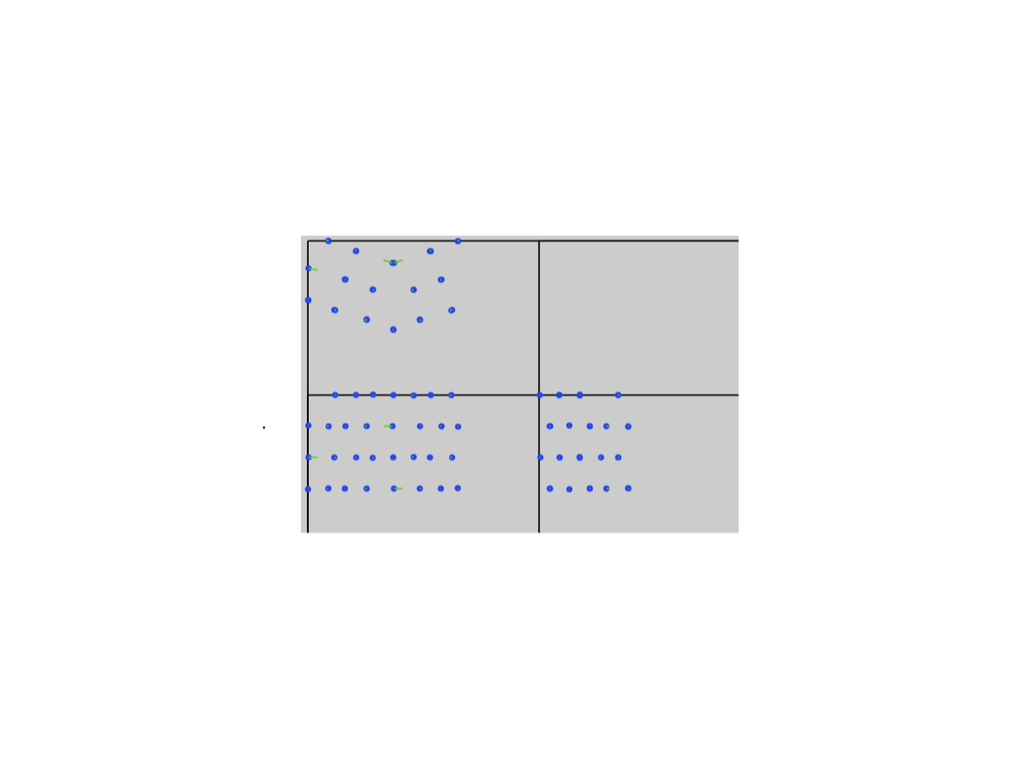
\includegraphics[width=10cm,bb= 0 0 937 753]{../figs/./boundary_narita.011.jpeg}
\caption{構造緩和前後による原子の移動を示した三面図.}
\label{fig:011}
\label{default}\end{center}\end{figure}

図中の緑線は,構造緩和をおこなう前後で各原子が移動した経路である.
この三面図はSVGで表示されているため,拡大しても解析度が落ちずに鮮明に描画することができ,原子の移動変化をより細かく見ることができる.
その結果,原子の正確な移動位置,並びに第一原理計算ソフトVASPによる系全体のエネルギーを計算する際の構造緩和に過ちが生じていないかを
容易に判断できるようになった.

\subsubsection{指定したz軸の層の白抜き表示}
POSCAR\_2223は4層の原子配列で構成されているため,原子配列を上から見た図,すなわち平面図では,原子同士が重なって配置してしまう.
したがって,指定した層の原子が平面図の中でどこに位置するのかを視覚的に確認するために原子の白抜き処理をおこなった.
白抜き処理は,読み込む2つのファイル名の後に白抜きする層の段階数を入れることで表示される.
層の段階数は上層から順に数字を割り振っており,分母が層の総数,分子が白抜きしたい層である.
以下の実行は,4層で構成されているPOSCAR\_2223の第1層目を白抜き処理する際に入力したものである.
\begin{lstlisting}[style=customCsh,basicstyle={\scriptsize\ttfamily}]
% ruby viewer.rb POSCAR_2223 POSCAR_2223_4 1/4
% open -a safari view.svg 
\end{lstlisting}
このときに表示された原子配列の三面図は.以下の図\ref{fig:012}である.

\begin{figure}[htbp]\begin{center}
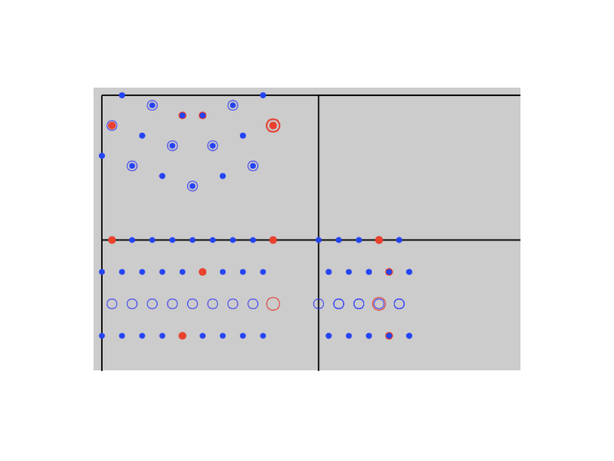
\includegraphics[width=8cm,bb= 0 0 937 753]{../figs/./boundary_narita.012.jpeg}
\caption{第一層目の原子を白抜きした三面図.}
\label{fig:012}
\label{default}\end{center}\end{figure}

この表示結果により,平面図と正面図の対応した位置が正確に判断できるだけでなく,図\ref{fig:013}のように平面図と側面図で対応した原子の位置を視覚的に判断することが可能になった.

\begin{figure}[htbp]\begin{center}
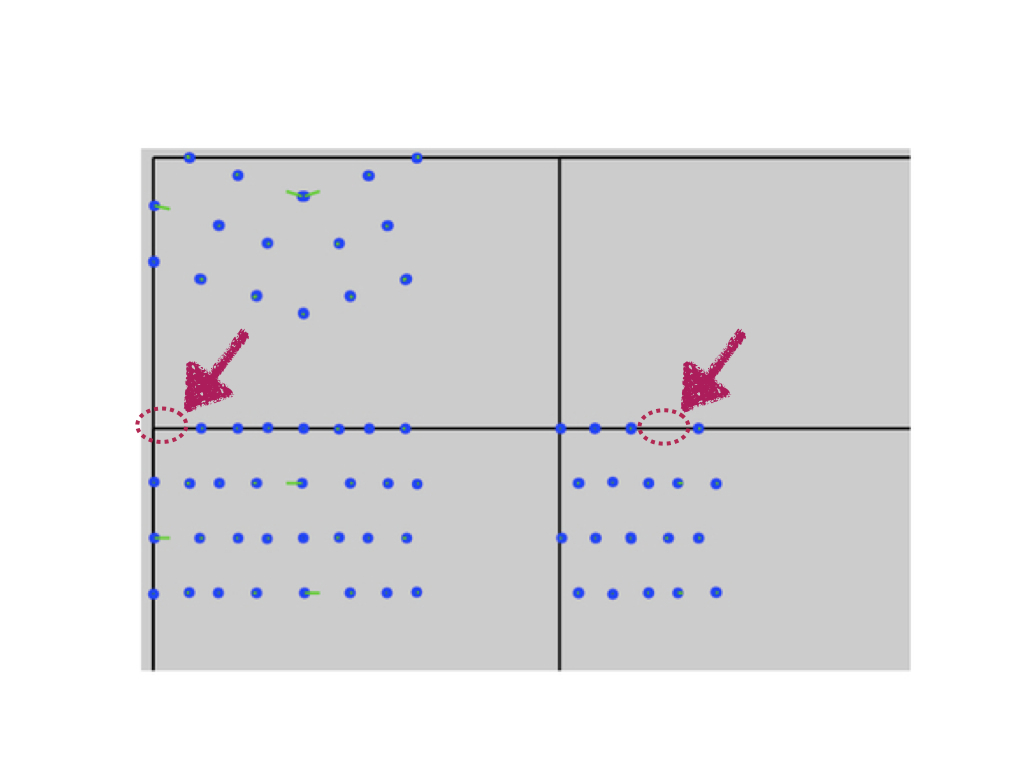
\includegraphics[width=8cm,bb= 0 0 937 753]{../figs/./boundary_narita.013.jpeg}
\caption{各図面の配置に対応していることを明示した図.}
\label{fig:013}
\label{default}\end{center}\end{figure}

なお,読み込む2つのファイル名の後に数値を入力しない,若しくは分子に0の値を入力することにより,白抜きなしの三面図を表示することが可能である.
\subsection{原子構造の改善点}
viewerによって三方向の視点で原子配列を表示した結果,構造緩和をおこなうためのPOSCARファイルに原子が一つ不足していることが分かった.
不足していた原子の位置は,図\ref{fig:014}の赤枠部分である.

\begin{figure}[htbp]\begin{center}
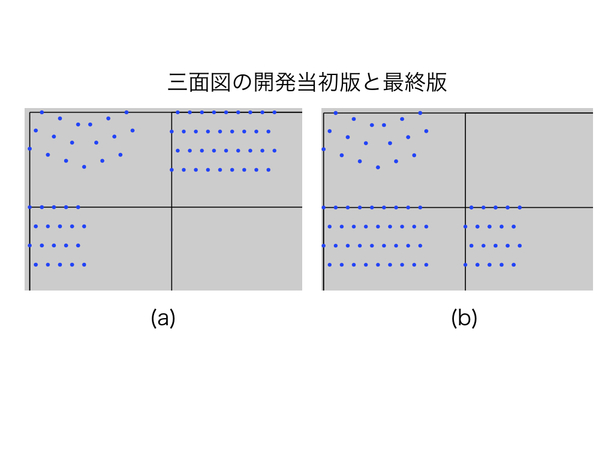
\includegraphics[width=8cm,bb= 0 0 937 753]{../figs/./boundary_narita.014.jpeg}
\caption{不足した原子を三面図で明示した図.}
\label{fig:014}
\label{default}\end{center}\end{figure}
この表示が,viewerによる計算,描画の誤りでないかを検証する必要があるため,ファイルPOSCAR\_afterの原子配列をVESTAで三次元化して確認をおこなった.
以下の図\ref{fig:015}は,構造緩和後のPOSCARファイルをVESTAで表示したものてある.

\begin{figure}[htbp]\begin{center}
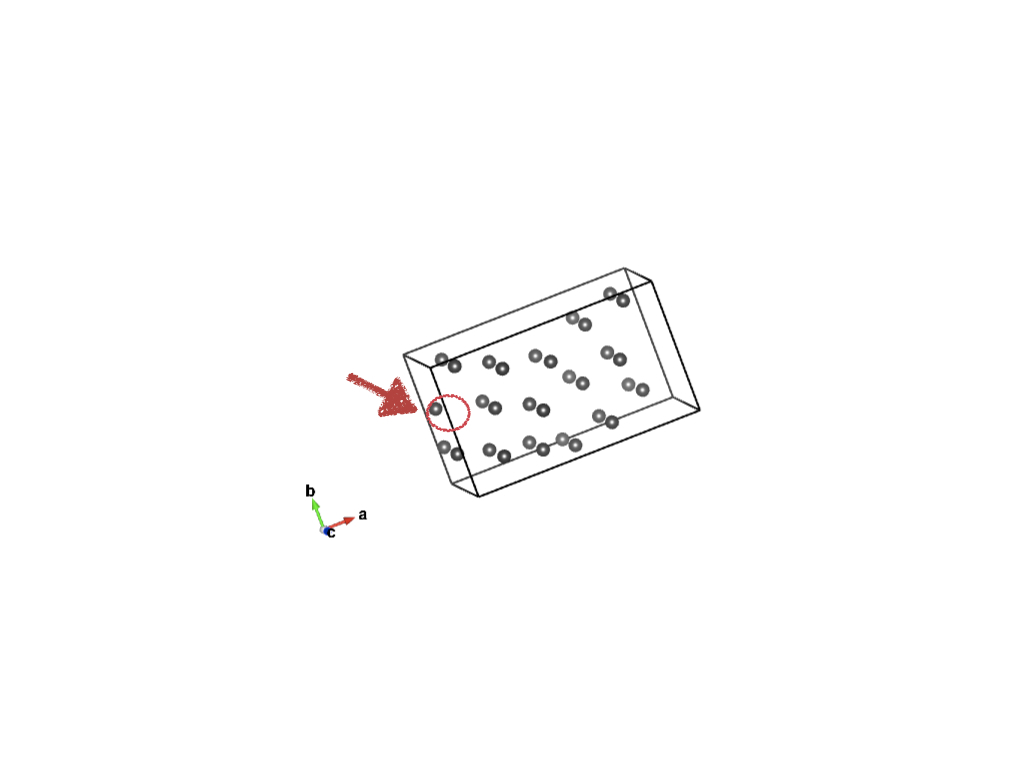
\includegraphics[width=11cm,bb= 0 0 937 753]{../figs/./boundary_narita.015.jpeg}
\caption{不足した原子をVESTAで視覚的に検証した図.}
\label{fig:015}
\label{default}\end{center}\end{figure}
その結果,図のように各々の位置で対応する原子がある中で,赤枠で括った部分には対応した原子が存在していないのが分かった.
したがって,三面図による不足した原子の発見はソフト内の過ちではないことが視覚的に立証できた.

\subsection{考察と今後の課題}
三面図を利用して原子配列を表示したことで,構造緩和をおこなう際に使用したPOSCARファイルに過ちがあったことに気づいた.
これは,今までの原子配列が結晶構造描画ソフト"VESTA"による三次元表示であり,原子の細かい位置が確認できず,原子が不足していることを認識できなかったためである.
したがって,粒界原子配列の構造緩和をおこなう計算を見直す必要がある.
また,本研究ではPOSCAR\_2223を基準として様々な描画を出力できるソフトを開発したが,より大きな粒界原子配列を視覚的に検証できるように改良していかなければならない.
さらに,三面図の配置では,正面図を物体の最も代表的な面と規定されているが,原子配列の表示で最も重要な面は,上から見た図,すなわち平面図であることが開発後に分かった.
したがって,今後は三面図の配置構成を図\ref{fig:016}のように変更して視覚的検証をおこなっていく.

\begin{figure}[htbp]\begin{center}
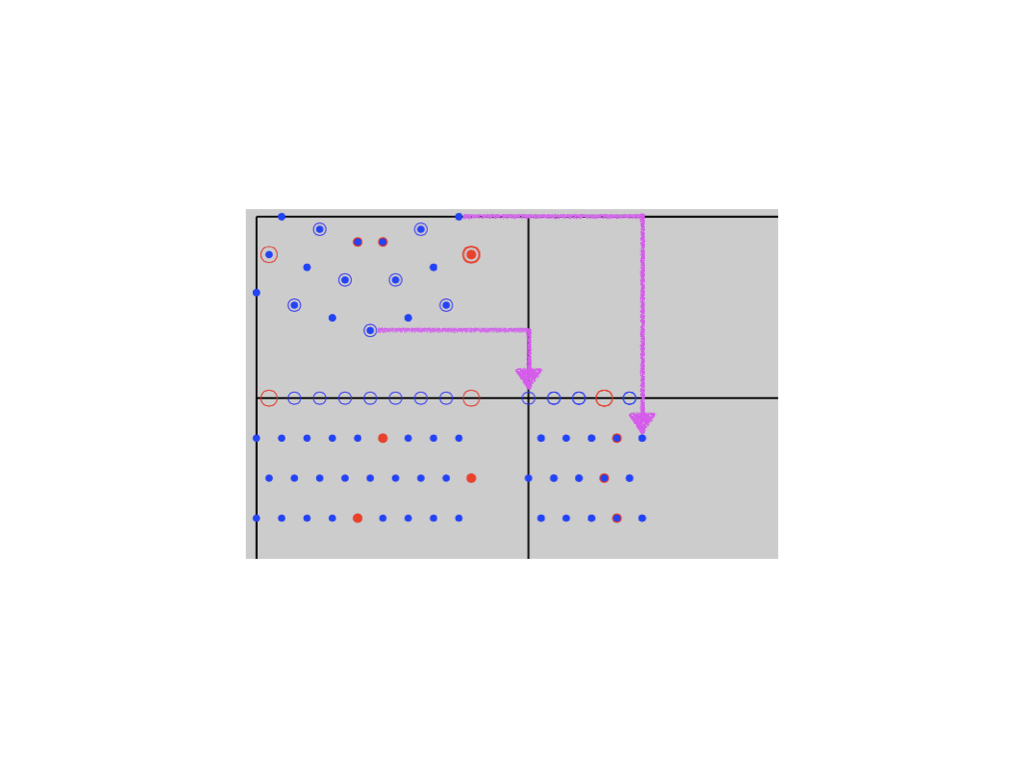
\includegraphics[width=12cm,bb= 0 0 937 753]{../figs/./boundary_narita.016.jpeg}
\caption{正面図と平面図の配置を変更した図.}
\label{fig:016}
\label{default}\end{center}\end{figure}
